\chapter{Implementation} \label{c:impl}

The VFIO implementation of Ixy.rs was used as a reference but was massively changed to fit the project structure and use case. The implementation for IOMMU support includes the initialization of the IOMMU, the steps needed to create mappings to the I/O virtual address space, and the access to the device registers. The complete code of the driver can be found on GitHub \cite{vroomsource}.

\section{Virtual Function I/O}
Virtual Function I/O (VFIO) is an IOMMU agnostic framework for exposing devices to userspace. VFIO acts like the kernel module to userspace drivers, allowing unprivileged, regulated access to physical memory and device registers.

As seen on \autoref{fig:layer-vfio}, VFIO consists of an IOMMU API for management of IOMMU mappings (VFIO backend) and a device API for device access, which uses the backend to perform the access. With the new introduction of IOMMUFD, the native backend of VFIO is considered the "legacy" backend. Legacy VFIO uses the type1 IOMMU API for x86 architectures or the SPAPR IOMMU API for ppc64 architectures. As our implementation is for x86, we will equate legacy VFIO with the type1 API.

The \texttt{vfio-pci} driver (device API) is used for interaction with the device, i.e., reading, writing, and mapping the device registers. Only the backend gets replaced when VFIO is used with IOMMUFD, as IOMMUFD still relies on \texttt{vfio-pci} to access device registers. We will first focus on the legacy VFIO implementation and then compare it to the implementation of IOMMUFD.
The layers of VFIO with both backends can be seen on \autoref{fig:layer}.

To use vroom with the IOMMU, we need to initialize the IOMMU, VFIO, DMA, and the NVMe device:
\begin{enumerate}
    \item \textbf{\nameref{sec:iommuinit}}: As the first step, the VFIO container for IOVAs is initialized. With this container and the NVMe IOMMU group, we obtain the device file descriptor.
    \item \textbf{\nameref{sec:pcieconfig}}: Using the device fd, we write to the PCIe configuration space to enable DMA and map the NVMe BAR to memory.
    \item \textbf{\nameref{sec:dmamapping}}: Using the container fd, we create a mapping in the IOMMU and, therefore, place it in the virtual address space of the NVMe controller for DMA.
    \item \textbf{\nameref{sec:nvmeinit}}: The final step is to initialize the NVMe controller for I/O operations.
\end{enumerate}

Interaction with the VFIO interface works using \texttt{ioctl} system calls.
\texttt{ioctl} or control device syscall, uses a file descriptor (\texttt{fd}), operation id (\texttt{op}), and optional arguments to perform actions on devices that are not covered by other system calls.
The operation IDs used for VFIO are defined as constants or enums in the \texttt{vfio.h} header file in the Linux kernel. To use these constants in Rust, they must be defined manually or with a crate like bindgen, which automates bindings for C and C++ libraries \cite{cratebindgen}. We chose the manual implementation to keep the binary and dependency list as small as possible.
Many \texttt{ioctl} calls used for VFIO also take in a mutable reference to a struct, which is used for specific input and output. These structs are also defined in \texttt{vfio.h} and can be ported over to Rust using the \texttt{\#[repr(C)]} attribute, which ensures the same struct alignment as in C.

To model the IOMMU, we implement the struct \texttt{Vfio} and the enum \texttt{VfioBackend}, as seen in \autoref{lst:vfiostructs}.
The shared functionality, e.g., accessing the device registers, is implemented on the struct \texttt{Vfio}, while the enum \texttt{VfioBackend} takes care of the backend-specific behavior, i.e., mapping DMA addresses.

\begin{minipage}{.95\linewidth}
    \begin{lstlisting}[language=Rust,caption={Structs used to model VFIO}, label=lst:vfiostructs]
    pub struct Vfio {
        pci_addr: String,
        device_fd: RawFd,
        page_size: Pagesize,
        iommu: VfioBackend,
    } 

    enum VfioBackend {
        Legacy {
            container_fd: RawFd,
        },
        IOMMUFD {
            ioas_id: u32,
            iommufd: RawFd,
        },
    }
\end{lstlisting}
\end{minipage}

\subsection{Groups and Containers}
VFIO works using (IOMMU-)groups and containers. Each group can contain one or multiple devices. As many devices use DMA between each other, a single IOMMU group has to be created, as these devices cannot function in an isolated environment. The other way round can also be the case, with one device exposing two interfaces, which get their own group each. Therefore, groups are the smallest unit that can be isolated by the IOMMU. While groups are supposed to provide the highest amount of isolation, the need for shared memory between devices often exists. This need can be solved by using containers. Containers consist of one or more groups. The groups in one container share the same I/O virtual address space created by the IOMMU, allowing both to access the same memory.
A new container can be created by opening the file \texttt{/dev/vfio/vfio}. The groups of devices bound to \texttt{vfio-pci} can be found under the path \texttt{/dev/vfio/\$GROUP}.

\subsection{Binding NVMe to \texttt{vfio-pci}}\label{sec:bindvfiopci}
To use the IOMMU for the driver, we first need to initialize the VFIO kernel module using \texttt{modprobe} and bind the \texttt{vfio-pci} driver to the NVMe device. By changing the owner of the container and group file to an unprivileged user, vroom can use the VFIO driver to create memory mappings and interact with the device without root.

\subsection{IOMMU container initialization}\label{sec:iommuinit}
To initialize the IOMMU, we first need to get the container file descriptor. The container is accessible under the path \texttt{/dev/vfio/vfio}. Using the raw container file descriptor, we can use the following \texttt{ioctl} calls:

\begin{lstlisting}[language=Rust, caption={\texttt{ioctl} calls needed for VFIO container initialization}, label=lst:containerioctls]
    ioctl_unsafe!(container_fd, VFIO_GET_API_VERSION)
    ioctl_unsafe!(container_fd, VFIO_CHECK_EXTENSION, VFIO_TYPE1_IOMMU)
    ioctl_unsafe!(group_fd, VFIO_GROUP_GET_STATUS, &group_status)
    ioctl_unsafe!(group_fd, VFIO_GROUP_SET_CONTAINER, &container_fd)
    ioctl_unsafe!(container_fd, VFIO_SET_IOMMU, VFIO_TYPE1_IOMMU)
    ioctl_unsafe!(group_fd, VFIO_GROUP_GET_DEVICE_FD, pci_addr)
    ioctl_unsafe!(container_fd, VFIO_IOMMU_GET_INFO, &iommu_info)   
\end{lstlisting}

Excluding the status and info calls, the functionality consists of initializing the IOMMU for the device groups by setting the container on the groups, enabling Type1 for the IOMMU, and fetching the device file descriptor. With the device file descriptor, we gain access to the device regions through the VFIO device API, allowing us to access the device registers.

\subsection{Device register access}\label{sec:pcieconfig}
Previously, device access was done through the \texttt{sysfs} (pseudo-)filesystem. \texttt{sysfs} exposes the device registers under the path \texttt{/sys/bus/pci/devices/\$PCI\_ADDRESS/}. As seen in \autoref{fig:pciconfig}, we need to access the command register and the NVMe BAR0 register. In \texttt{sysfs}, these are the \texttt{config} and \texttt{resource0} files in the device directory. The \texttt{config} file points to the address 0x0 of the PCI configuration space. By adding the command register offset (0x4), we can access the command register.

Using the offset 0x2 in the command register, we can set the bit for bus mastering, allowing the device to perform DMA.
To map the BAR0 register to memory, we can use \texttt{mmap} with a file descriptor to \texttt{resource0}.

To do the same using VFIO, we use the VFIO device API.
We can access the device registers using the \texttt{VFIO\_DEVICE\_GET\_REGION\_INFO} \texttt{ioctl} operation on the device fd. This operation requires the struct \texttt{vfio\_region\_info} as the third parameter, which needs to be initialized with a given index from \texttt{vfio.h}.
We use the indices \texttt{VFIO\_PCI\_CONFIG\_REGION\_INDEX} and \texttt{VFIO\_PCI\_BAR0\_REGION\_INDEX} to access the config and BAR register respectively. The struct is used as an input/output struct. After
After performing the syscall, the other fields are set, e.g., size or offset, and can be used to read/write or memory map device registers.

Using \texttt{VFIO\_PCI\_CONFIG\_REGION\_INDEX} as the index, we again get the PCIe configuration space address 0x0. By adding the command register offset, we can set the bus mastering bit to enable DMA.
After this, we can map the NVMe base address register to memory using the \texttt{VFIO\_PCI\_BAR0\_REGION\_INDEX} index.
The offset and size can be directly passed into \texttt{mmap} to map the BAR0 register to memory, as seen on \autoref{lst:bar0map}.

\begin{minipage}{.95\linewidth}
    \begin{lstlisting}[language=Rust,caption={Mapping the BAR0 NVMe register to memory}, label=lst:bar0map]
let mut region_info = vfio_region_info {
    argsz: mem::size_of::<vfio_region_info>() as u32,
    flags: 0,
    index: Self::VFIO_PCI_BAR0_REGION_INDEX,
    cap_offset: 0,
    size: 0,
    offset: 0,
};

ioctl_unsafe!(
    self.device_fd,
    IoctlOp::VFIO_DEVICE_GET_REGION_INFO,
    &mut region_info
)?;

let len = region_info.size as usize;

let ptr = mmap_unsafe!(
    ptr::null_mut(),
    len,
    libc::PROT_READ | libc::PROT_WRITE,
    libc::MAP_SHARED,
    self.device_fd,
    region_info.offset as i64
)?; 
\end{lstlisting}
\end{minipage}

\subsection{DMA (Un-)Mapping}\label{sec:dmamapping}
When using physical addresses for DMA, several steps have to be performed to ensure that the page is not moved. Firstly, hugepages must be used, as the kernel cannot move these. The allocated memory is also locked using \texttt{mlock} to prevent the page from being swapped out of memory. The hugepage file is created in the directory where hugetlbfs is mounted, in our case \texttt{/mnt/huge}. By using \texttt{mmap} with the file descriptor and locking it, we can create a statically mapped page in memory. To get the physical address for DMA, the address translation entry in the MMU needs to be fetched from \texttt{/proc/self/pagemap}. As \texttt{mmap} uses \qty{4}{\kibi\byte} by default, we have to specify the use of hugepages with the \texttt{MAP\_HUGETLB} flag. The resulting pagesize depends on the default hugepage size of the system but can be specified with either the \texttt{MAP\_HUGE\_2MB} or the \texttt{MAP\_HUGE\_1GB} flag.

As seen in \autoref{lst:mapdma}, VFIO greatly simplifies this, as using IOVAs alleviates the need for ensuring the physical address does not change. This is handled by VFIO. Firstly, we can either allocate or map a file to the process virtual space using \texttt{mmap}. As we do not have the restriction of using hugepages, we can also perform the mapping using the default \qty{4}{\kibi\byte} pages.
To get the IOVA for a corresponding page in memory, we need to use the \texttt{vfio\_iommu\_type1\_dma\_map} struct with the VFIO operation \texttt{VFIO\_IOMMU\_MAP\_DMA}. To map an address correctly, we need to specify the address mapping in the struct. \texttt{vaddr} is the address in the process virtual address space, i.e., the address returned by \texttt{mmap}. By setting the field \texttt{iova} to the same address, we can conveniently use the same address for the IOVA. We do this to avoid manually managing the IOVAs. Finally, the size has to be specified to the length passed to \texttt{mmap}. In the \texttt{flags} field, we can specify if the memory is accessible with read and/or write. By default, we set both. This IOVA can then be used just like the physical address by the NVMe controller.

\begin{minipage}{.95\linewidth}
    \begin{lstlisting}[language=Rust,caption={Mapping memory for DMA}, label=lst:mapdma]
    let mut iommu_dma_map = vfio_iommu_type1_dma_map {
        argsz: mem::size_of::<vfio_iommu_type1_dma_map>() as u32,
        flags: IoctlFlag::VFIO_DMA_MAP_FLAG_READ 
                | IoctlFlag::VFIO_DMA_MAP_FLAG_WRITE,
        vaddr: ptr as u64,
        iova: ptr as u64,
        size,
    };

    ioctl_unsafe!(
        *container_fd,
        IoctlOp::VFIO_IOMMU_MAP_DMA,
        &mut iommu_dma_map
    )?;

    let iova = iommu_dma_map.iova as usize; 
\end{lstlisting}
\end{minipage}

\paragraph{Unmapping DMA}
The implementation includes a function for unmapping IOVAs. As the mappings automatically get unmapped when the driver exits, it is still nice to have when repeatedly mapping huge files. Using the \texttt{VFIO\_IOMMU\_UNMAP\_DMA} \texttt{ioctl} operation, we can unmap the memory and finally free it using \texttt{munmap}.

\subsection{NVMe initialization}\label{sec:nvmeinit}
Using the mapped NVMe BAR and the ability to create DMA mappings, we can now initialize the NVMe controller. This mainly consists of allocating the queues and mapping them to be accessed by the NVMe controller through DMA. The IOVAs of the admin queues can be written to the mapped BAR. The BAR is also used to configure the NVMe, e.g., setting the queue entry sizes. When the NVMe is configured and ready, an I/O queue pair can be created using the admin queues.

\subsection{I/O operations with VFIO}
After initialization, the NVMe is ready to use. An example for an I/O operation is shown in \autoref{fig:vroom-graph}.
\begin{figure}[H]
    \centering
    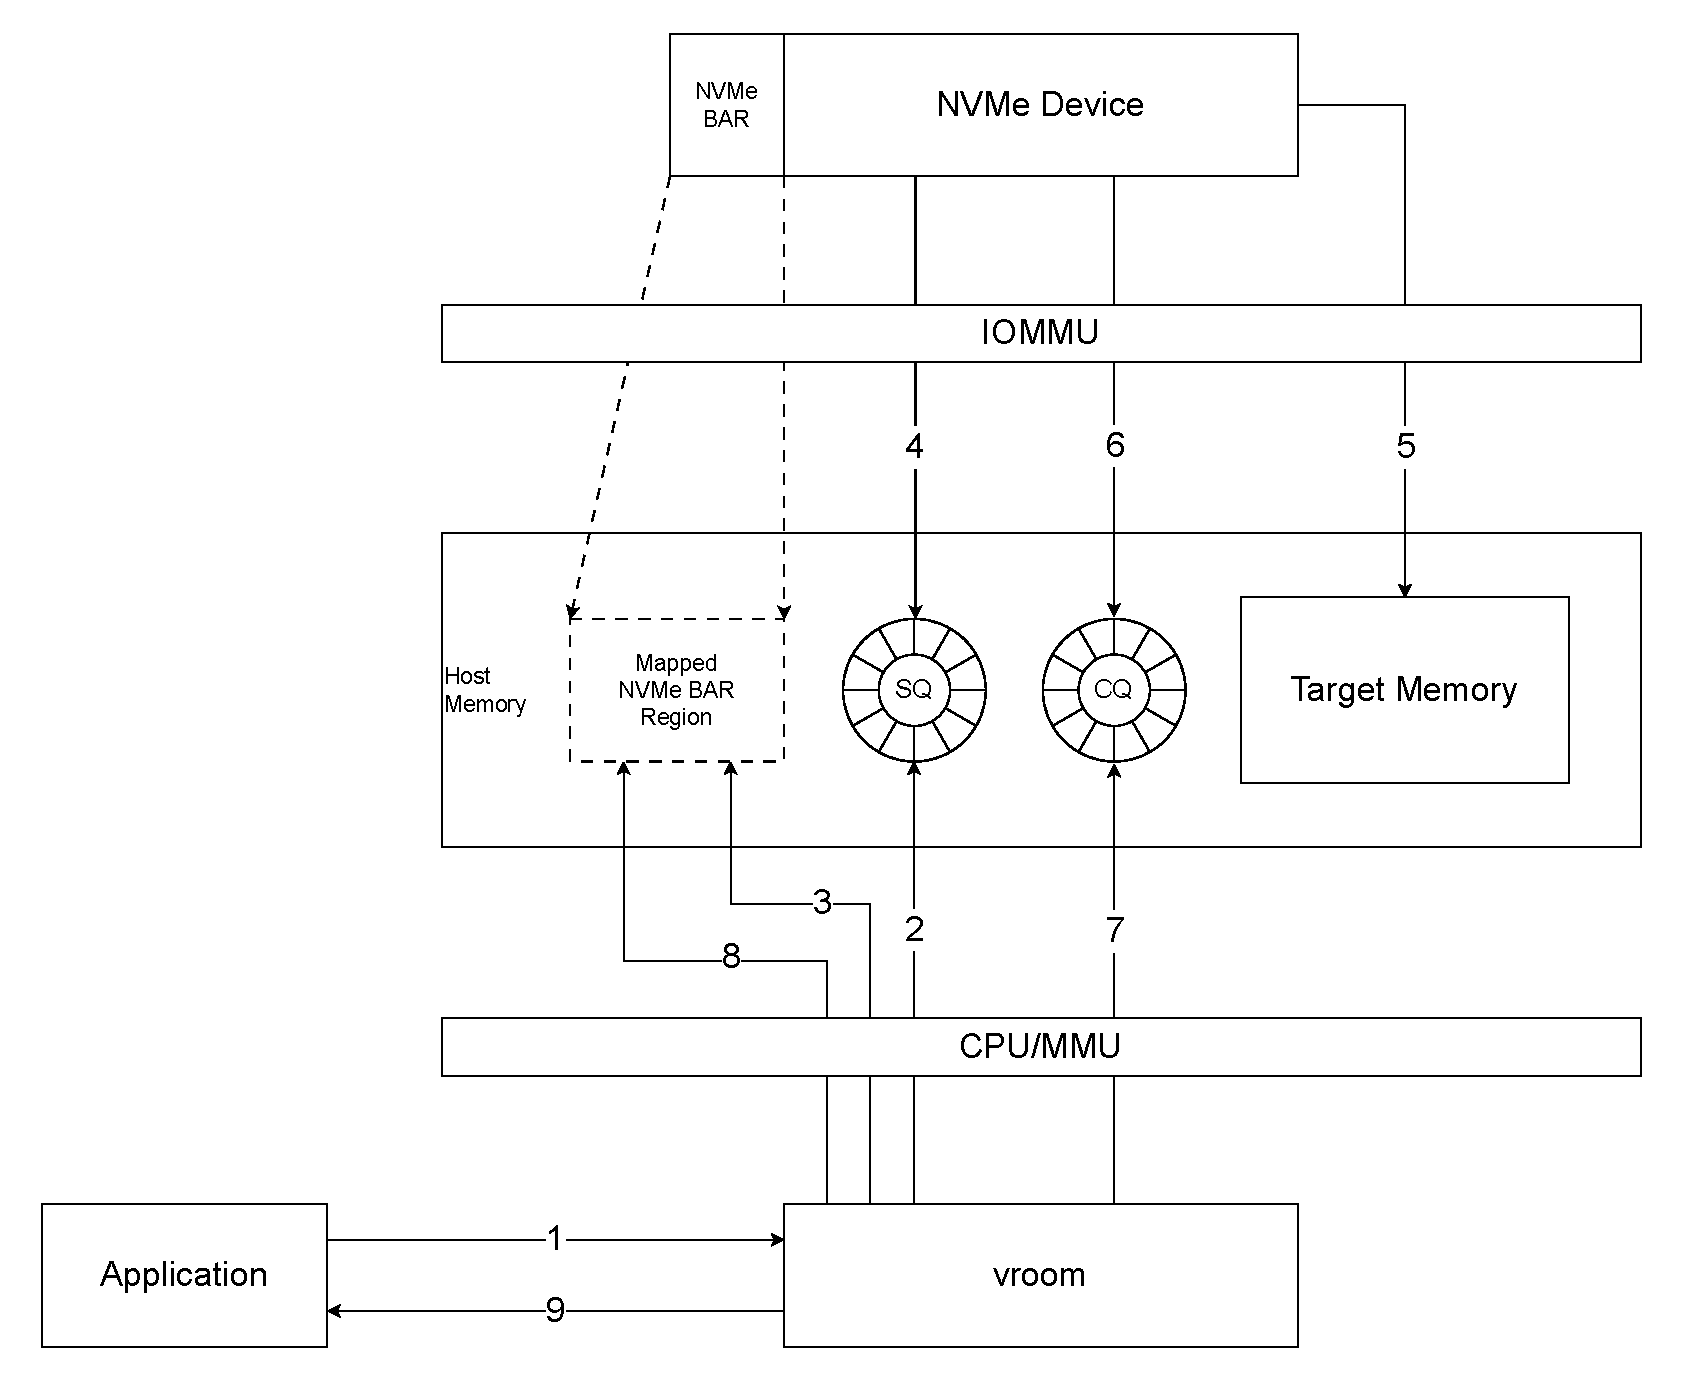
\includegraphics[width=\textwidth]{figures/vroomdiagram.pdf}
    \caption{I/O operation using vroom with enabled IOMMU}
    \label{fig:vroom-graph}
\end{figure}
The sequence of events in \autoref{fig:vroom-graph} are as followed:
\begin{enumerate}
    \item \textbf{I/O function call:} The application calls a read/write method on vroom
    \item \textbf{Command Submission:} vroom creates a \texttt{NvmeCommand} struct and places it on the Submission Queue (SQ) head.
    \item \textbf{Ring SQ Doorbell:} vroom places the submission queue head address in the doorbell register in the mapped NVMe BAR.
    \item \textbf{Take Command:} The NVMe takes the command from the SQ using DMA.
    \item \textbf{Perform I/O:} The NVMe uses the IOMMU to access the host memory via DMA and performs the read/write command.
    \item \textbf{Complete I/O:} The NVMe uses DMA to place a \texttt{NvmeCompletion} struct instance on the head of the Completion Queue (CQ).
    \item \textbf{Polled CQ:} By polling the CQ, vroom can process the CQ entry.
    \item \textbf{Ring CQ Doorbell:} After processing the CQ entry, vroom rings the CQ Doorbell to notify the NVMe controller that the Completion Queue has been processed.
    \item \textbf{Notify application :} vroom notifies the application of the success of the I/O operation. The application can continue running.
\end{enumerate}

\section{IOMMUFD}
The IOMMU File Descriptor user API (IOMMUFD) offers a way of controlling the IOMMU subsystem using file descriptors in userspace \cite{iommufdkerneldocs}. IOMMUFD offers a more granular management of the IOMMU, using devices instead of groups. Additionally, it supports a more user-friendly interface, allowing the user to manage IOVAs easily. Although IOMMUFD could be used as a standalone to provide simple IOMMU functionality like mapping or unmapping, it is not suited userspace drivers without VFIO. Device registers still need to be accessed through the \texttt{vfio-pci} driver. Consequently, IOMMUFD is used with VFIO, replacing its backend, i.e., the interaction with the IOMMU, but still relying on the functionality of parts of VFIO.
IOMMUFD was only recently added to the Linux Kernel in December 2022. For example, Debian 12 does not include it. Considering that it is not widely available or enabled on many distributions, our driver offers both options of using the IOMMU.
Instead of containers or groups, IOMMUFD uses I/O address spaces (IOAS) and character device file descriptors. Just like containers, IOAS can be used to provide shared memory mappings for multiple devices. Implementing IOMMUFD is similar to VFIO, but there are some key differences.
As with VFIO, to interact with IOMMUFD, we use the syscall \texttt{ioctl}. The needed bindings, flags, and operations are defined in the Linux kernel under the path \texttt{include/uapi/linux/iommufd.h}. Again, we manually port the needed structs and constants to Rust.

The first change is the acquisition of the group/device and the container/IOMMU fd.
In VFIO, a container can be created using the file \texttt{/dev/vfio/vfio}. For IOMMUFD, the iommu fd must first be acquired from \texttt{/dev/iommu}. Using the \texttt{IOMMU\_IOAS\_ALLOC} \texttt{ioctl}, a new IOAS can be allocated.
The device file descriptor, which was previously acquired with \texttt{VFIO\_GROUP\_GET\_DEVICE\_FD}, can now simply be obtained through opening the character device \texttt{/dev/vfio/devices/vfioX} \cite{vfiokerneldocs}. In order to use the device with VFIO, it still has to be bound to IOMMUFD, using \texttt{VFIO\_DEVICE\_BIND\_IOMMUFD}.

The IOAS can then be assigned to the device using \texttt{VFIO\_DEVICE\_ATTACH\_IOMMUFD\_PT}. As with containers, this operation can be performed on multiple devices for a shared IOAS. The equivalent in VFIO is \texttt{VFIO\_GROUP\_SET\_CONTAINER}.

When using VFIO with IOMMUFD, the interaction with \texttt{vfio-pci} stays the same. Primarily, the functionality of reading, writing, and mapping to the device registers is unchanged, except that instead of the VFIO device fd, the character device fd is used.

As for (un-)mapping DMA, the \texttt{IOMMU\_IOAS\_MAP} and \texttt{IOMMU\_IOAS\_UNMAP} are used instead of \texttt{VFIO\_IOMMU\_MAP\_DMA} and \texttt{VFIO\_IOMMU\_UNMAP\_DMA}.

\begin{minipage}{.95\linewidth}
    \begin{lstlisting}[language=Rust,caption={Mapping memory for DMA with IOMMUFD}, label=lst:mapdmaiommufd]
    let mut ioas_map = iommu_ioas_map {
        size: mem::size_of::<iommu_ioas_map>() as u32,
        flags: IoctlFlag::IOMMU_IOAS_MAP_WRITEABLE | IoctlFlag::IOMMU_IOAS_MAP_READABLE,
        ioas_id: *ioas_id,
        __reserved: 0,
        user_va: ptr as u64,
        length: size as u64,
        iova: 0,
    };

    ioctl_unsafe!(*iommufd, IoctlOp::IOMMU_IOAS_MAP, &mut ioas_map)?; 

    let iova = ioas_map.iova as usize; 
\end{lstlisting}
\end{minipage}

\begin{figure}[H]
    \centering
    \subcaptionbox {VFIO with Containers \label{fig:layer-vfio}} {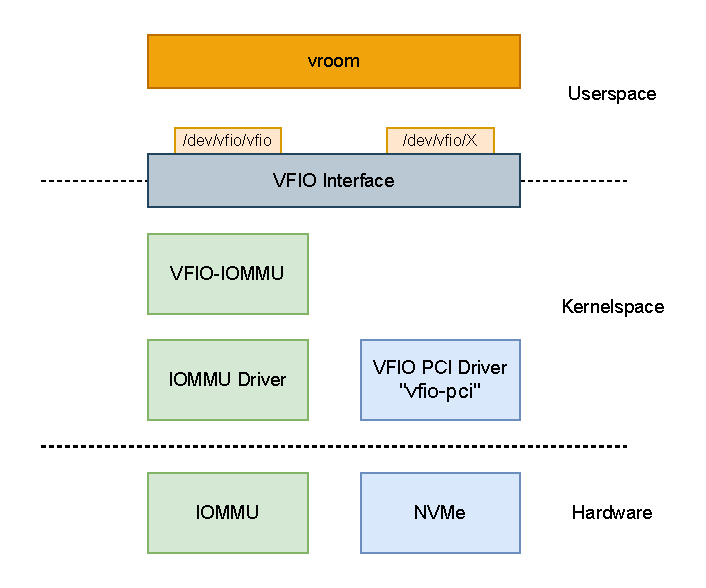
\includegraphics[width=0.67\textwidth]{figures/VFIOLayer.pdf}}
    \subcaptionbox {VFIO with IOMMUFD (IOAS) \label{fig:layer-iommufd}} {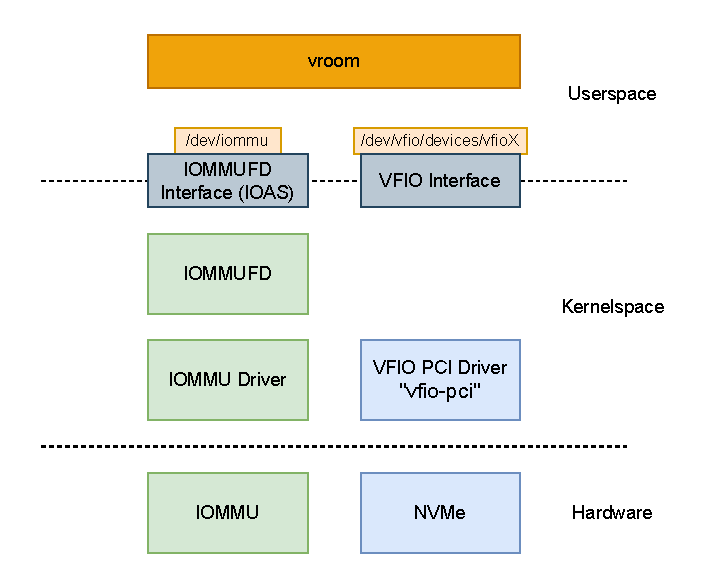
\includegraphics[width=0.67\textwidth]{figures/IOMMUFDLayer.pdf}}
    \caption{Layer diagrams of VFIO with VFIO Container API and IOMMUFD, adapted from \cite{dpdkiommufd}}
    \label{fig:layer}
\end{figure}

\section{Linux Systemcalls}
A variety of Linux Systemcalls (syscalls) are used in vroom. The syscalls that are used by vroom are \texttt{mmap}, \texttt{ioctl}, \texttt{pread}, \texttt{pwrite} (and \texttt{mlock} for the non-IOMMU version). While there are crates that implement the syscall functionality, we only use the \texttt{libc} crate to avoid inflating the dependency list and executable size. As these require C-like syntax and unsafe code in Rust, we implement wrapper macros to provide locality of behavior and secure error handling. In \autoref{lst:mmapmacro}, the macro for the \texttt{mmap} syscall can be seen.
As part of our error handling, we introduce an error enum variant for each syscall. To not hide the innate unsafety of these macros, we add the suffix "\_unsafe".

\begin{lstlisting}[language=Rust,caption={Syscall \texttt{mmap} macro, with own error variant}, label=lst:mmapmacro]
    #[macro_export]
    macro_rules! mmap_unsafe {
        ($addr:expr, $len:expr, $prot:expr, $flags:expr, $fd:expr, $offset:expr) => {{
            let ptr = unsafe { libc::mmap($addr, $len, $prot, $flags, $fd, $offset) };
            if ptr == libc::MAP_FAILED {
                Err(Error::Mmap {
                    error: (format!("Mmap with len {} failed", $len)),
                    io_error: (std::io::Error::last_os_error()),
                })
            } else {
                Ok(ptr)
            }
        }};
    } 
\end{lstlisting}
